\documentclass{article}
\usepackage{geometry}
 \geometry{
 a4paper,
 total={170mm,257mm},
 left=20mm,
 top=20mm,
 }
\usepackage[utf8]{inputenc}
\usepackage[T1]{fontenc}
\usepackage[english]{babel}
\usepackage[language=english, style=numeric, sorting=none]{biblatex}
\usepackage{lipsum}
\usepackage{hyperref}
\hypersetup{
    colorlinks=true,
    linkcolor=blue,
    filecolor=magenta,      
    urlcolor=cyan,
}

\newcommand{\lecture}[2]{
  \pagestyle{myheadings}
  \thispagestyle{plain}
  \newpage
%   \setcounter{lecnum}{#1}
  \setcounter{page}{1}
   \noindent
   \begin{center}
   \framebox{
      \vbox{\vspace{2mm}
    \hbox to 6.28in { {\bf ELP 305: Design and Systems Laboratory
        \hfill Semester II 2020-2021} }
       \vspace{4mm}
       \hbox to 6.28in { {\Large \hfill Laboratory Report #2, Group H: #2  \hfill} }
       \vspace{2mm}
       %\hbox to 6.28in { {\it Course Coordinator: Prof. S. D. Joshi \hfill} }
      \vspace{2mm}}
   }
   \end{center}
   % Write your entry numbers here
    %\vspace{2mm}\\
    \noindent
    %{\bf Name}: {Arunava Das} \hfill {\bf Entry No}: {2018EE10593}
    %\vspace{2mm}\\
    \noindent
    {\bf Note}: {\it LaTeX template courtesy of UC Berkeley EECS dept.\cite{noauthor_latex_nodate}}
    
   \vspace*{10mm}
}

% ADD YOUR PACKAGES HERE
\usepackage{amsmath,amsfonts,graphicx,courier,listings,float}



% ADD YOUR REFERENCES IN THIS FILE
\addbibresource{ref.bib} 

\newtheorem{theorem}{Theorem}
\newtheorem{proposition}{Proposition}

\begin{document}
\lecture{1}{February 27}

\begin{tabular}{ |p{0.7cm}|p{5cm}|p{3.1cm}|p{6cm}|  }
 \hline
 \multicolumn{4}{|c|}{\textbf{\textit{Members of the group H}}} \\
 \hline
 \hline
 Sl & \textbf{Position} & \textbf{Entry Number} & \textbf{Name}\\
 \hline
 \hline
1 & \textbf{Lead Coordinator} & 2018EE10593 & Arunava Das \\ \hline
2 & Requirements Coordinator & 2018EE30610 & Harsh Wardhan \\ \hline
3 & Specifications Coordinator & 2018MT10737 & Akshat Rao \\ \hline
4 & Specifications Coordinator & 2018EE10603 & Dedeepyo Ray \\ \hline
5 & Electrical Design Coordinator & 2018MT60798 & Zuhaib ul Zamann \\ \hline
6 & Electrical Design Coordinator & 2018EE10499 & Shashank Goyal \\ \hline
7 & Mechanical Design Coordinator & 2018MT60795 & Snehil Grandhi \\ \hline
8 & Mechanical Design Coordinator & 2018EE10459 & Chathur Gudesa \\ \hline
9 & Documentation Coordinator & 2018MT10759 & M Santosh \\ \hline
10 & Documentation Coordinator & 2018MT10756 & Ishant Bhaskar \\ \hline
11 & Member & 2018EE30534 & Darpan Kumaryadav \\ \hline
12 & Member  & 2018EE30538 & Dharmendra Seervi \\ \hline
13 & Member & 2018EE30543 & Himanshu Gaud \\ \hline
14 & Member & 2018MT60793 & Satendra Singhparashar \\ \hline
15 & Member  & 2018EE10494 & Rohit Agarwal \\ \hline
16 & Member & 2018EE30598 & Bharat Runwal \\ \hline
17 & Member & 2018MT60790 & Ravi Pushkar \\ \hline
18 & Member & 2018MT60788 & Ramneek Singhgambhir \\ \hline
19 & Member & 2018MT60776 & Aakash Garg \\ \hline
20 & Member & 2018EE10189 & Aditya Bansal \\ \hline
21 & Member & 2018MT60787 & Prateek Singh \\ \hline
22 & Member & 2018MT60786 & Pranaav \\ \hline
23 & Member & 2018MT60779 & Bhupender Dhaka \\ \hline
24 & Member & 2018EE10491 & Ranajay Medya \\ \hline
25 & Member & 2018MT60791 & Rishu Raj \\ \hline
26 & Member & 2018MT60777 & Adwaith H Sivam \\ \hline
27 & Member & 2018MT10770 & Subhalingam D \\ \hline
28 & Member & 2018EE10483 & Penumudinagavenkata Saiabhinay \\ \hline
29 & Member & 2018MT10740 & Anirudha Akela \\ \hline
30 & Member	& 2018EE30569 & Yerukula Sravanasai \\ \hline
31 & Member	& 2018EE30558 & Reddy Cihir \\ \hline
32 & Member	& 2018MT60778 &	Ashwini Kumar \\ \hline
33 & Member	& 2018MT10745 & Aryan Gupta \\ \hline
34 & Member	& 2018MT60244 & Shaurya Goyal \\ \hline
35 & Member	& 2018MT10763 & Punit Shyamsukha \\ \hline
36 & Member	& 2018MT10760 & Mukul Kumar \\ \hline
37 & Member	& 2018MT60797 & Vishal Meena \\ \hline
38 & Member	& 2018EE10514 & Vikas Kumar \\ \hline
39 & Member	& 2018MT60199 & Anshul Tak \\ \hline
40 & Member	& 2018EE10456 & Biruduraju Harahima dhruthi  \\ \hline
\end{tabular}

\section{Requirements for the circuit}

\subsection{Electrical requirements}


The device needs:
\begin{itemize}
    \item To input 220V- 50Hz AC supply and supply a regulated 5V DC output. 
    \item To be able to function in a wide Voltage range (180-260V AC, 50Hz).
\end{itemize}


To achieve these requirements, the following components\cite{noauthor_diy_nodate} were used to make the charger :

\begin{enumerate}
    \item One 220V / 12V step-down transformer (turns ratio of 55:3) 
    \item Four 1N4007 diodes (used in the rectifier)
    \item One electrolytic capacitor of capacitance 22mF and one unpolarized capacitance of 1$\mu$F respectively.

    \item One IC LM7805.
\end{enumerate}

\subsection{Mechanical requirements}
The device needs to:
\begin{itemize}
    \item be reliable, intuitive, compact, safe and easy to use. 
    \item Output over a standardized interface such as USB 2.0 / USB-C / USB-3PD.
    \item be able to function in a wide variety of temperatures and environmental factors.
\end{itemize}
For these reasons, the following mechanical components are being planned to be included :

\begin{enumerate}
    \item A Male Pin to attach to the Switchboard plug (IS:1293) 
    \item One USB cable, single-strand, of 1m length, at-least double wired and of 22 AWG.
    \item One USB type C male port
    \item One heat sink (according to the IC used)
    \item One PCB board (52x84 mm)
    \item The device needs to be compact, safe and reliable enough to use. 
    \item The device needs to operate in a wide temperature range (-20C to 60C) and across wide ranges of other environmental factors.  
\end{enumerate}

\section{Selection of Components}

\subsection{Capacitors}

The capacitor C1 is used to minimize ripple in output voltage of rectifier. The minimum capacitance required varies inversely as operating frequency and voltage ripple magnitude, and directly as the DC value of the output voltage, along with a constant. By trial and error, 22mF at C2 give reasonably low ripple for all the input voltages. The output capacitor C1 of 1$\mu$F helps stability and transient response in output.\cite{noauthor_smps_nodate}

\subsection{Diodes}

1N400X series of diodes\cite{noauthor_1n4001-1n4007_nodate} are fairly common in rectifier circuits. 1N4007 has the highest DC blocking voltage, i.e, maximum reverse voltage, among these. It can thus handle high voltages quite easily. To allow for large deviations (undesired but as a safety measure) 1N4007 is used. 

\subsection{Integrated Circuits}

The LM78XX family of ICs\cite{noauthor_lm7805_nodate} provide a constant DC output voltage. The XX represents the value of this voltage in Volts. It can be operated for output current of 1.5A DC also (and beyond too with proper considerations, limited by 2.4A) within 150 degrees Celsius. C2 control the ripple to keep the IC's input voltage within tolerance limits. Thus, it is commonly used as a voltage regulator.

\subsection{Transformer}

A transformer was specified in LTSpice\cite{noauthor_transformer_nodate} with two inductors coupled together at coupling coefficient 1 and in accordance with the equation,

\begin{equation}
 \frac{L_{primary}}{L_{secondary}} = {(\frac{N_{primary}}{N_{secondary}})}^2 = {(\frac{V_{primary}}{V_{secondary}})}^2   
\end{equation}

taking primary and secondary to be 220V AC and 12V AC respectively.
While actual designing, we will have to look into the voltage and current ratings of the transformer, generally available in dimensions 42x38mm.
\begin{figure}[h!]
\centerline{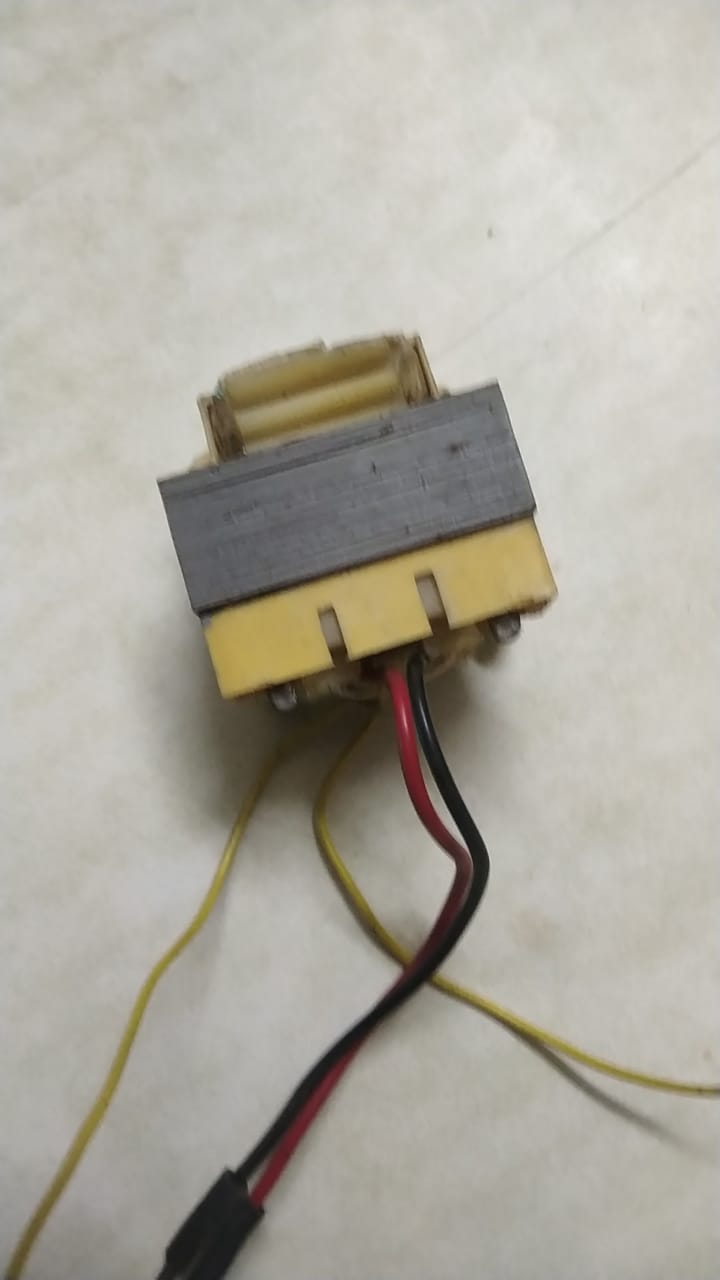
\includegraphics[scale=.2]{Images/ab.jpeg}}
\caption{Transformer to be used, left as a square blank space in the PCB}
\label{figb}
\end{figure}



\section{Specifications}

The mobile phone charger demanded 5V DC output voltage and 1A DC output current. Hence, a load drawing constant 1A current was added to the circuit in parallel with the output capacitor and diode. The AC mains was modelled by a voltage source producing a sinusoidal voltage wave of 220V (RMS), in series with a small source resistance of 1m Ohms. 

The circuit acts sequentially:
\begin{enumerate}
    \item The mains supply voltage is stepped down to 12 V (range - 11.68-12.4V).
    \item A full-wave rectifier is used to convert this to a DC voltage.
    \item Ripples in output voltage of rectifier are removed by using a large capacitor in parallel with a polar capacitor.
    \item The filtered voltage is fed to LM7805\cite{noauthor_what_nodate}\cite{noauthor_buck_nodate} which outputs constant DC value of 5V.
    \item The external load draws a constant 1A current.
\end{enumerate}

\begin{figure}[h!]
\centerline{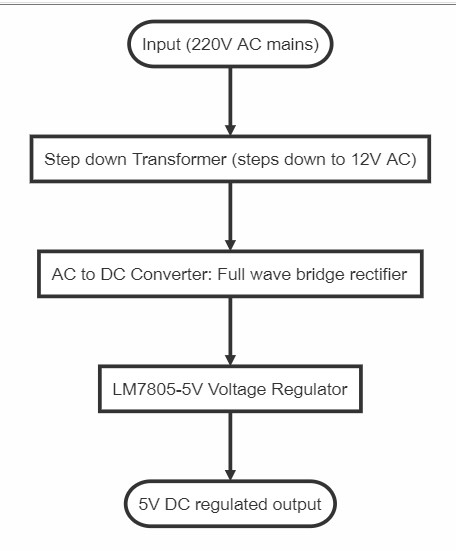
\includegraphics[scale=.55]{Images/flowchart.jpg}}
\caption{Circuit schematic}
\label{figb}
\end{figure}

\newpage
\subsection{Circuit schematic diagram}

\begin{figure}[h!]
\centerline{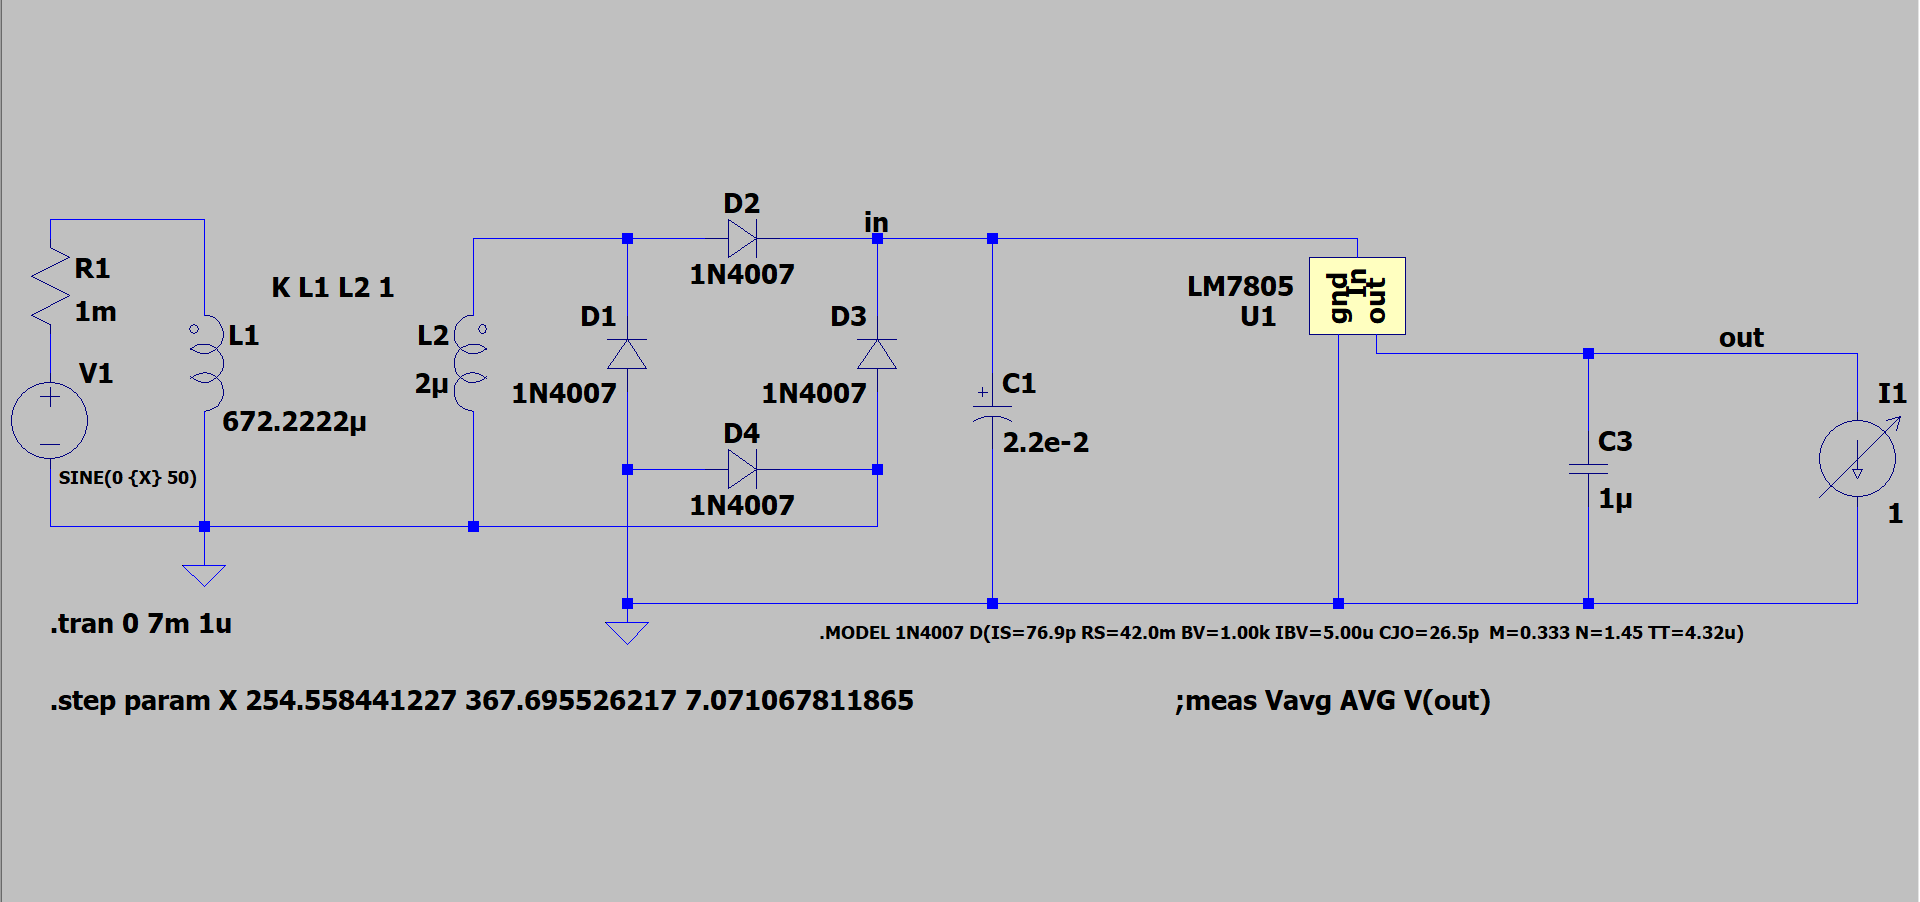
\includegraphics[scale=.4]{Images/1.PNG}}
\caption{Circuit schematic}
\label{figb}
\end{figure}


\subsection{Simulation of regulated DC output}

The output voltage at input voltage of 230V AC (RMS) was plotted. 

\begin{figure}[h!]
\centerline{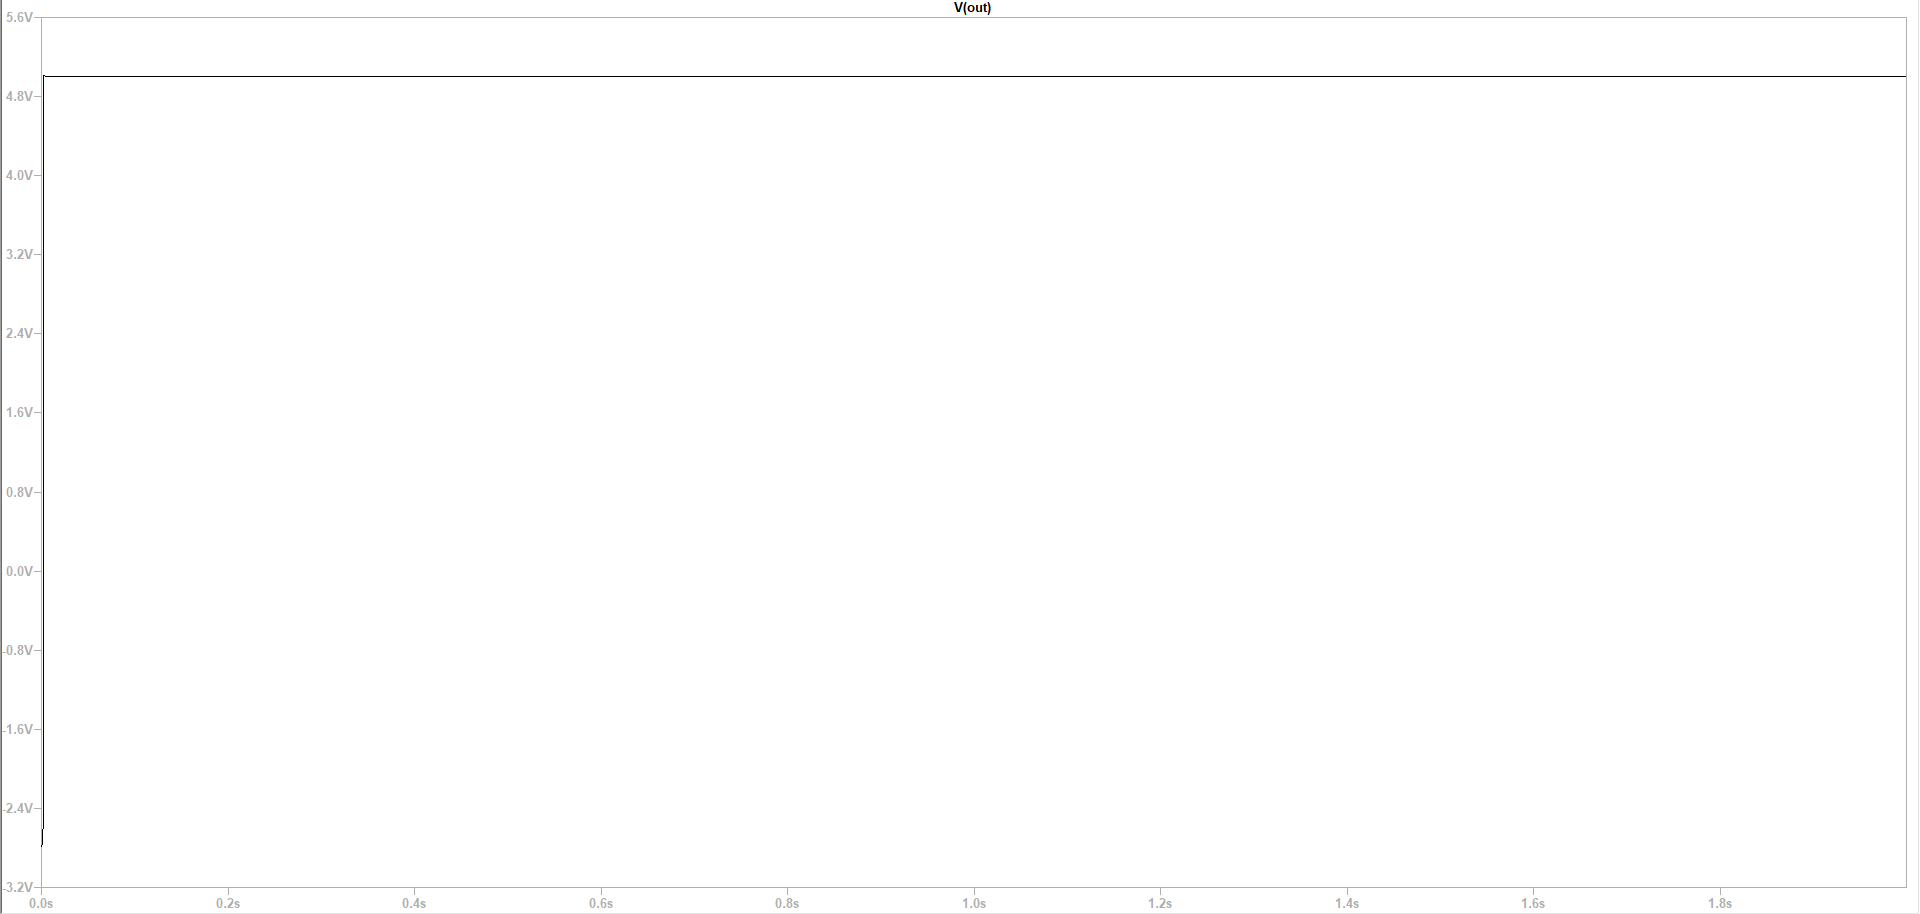
\includegraphics[scale=.4]{Images/2.PNG}}
\caption{V(Out) settling times}
\label{figb}
\end{figure}

It was found to settle at 5V DC.

The input voltage to the LM7805 was plotted. 

\newpage
\begin{figure}[h!]
\centerline{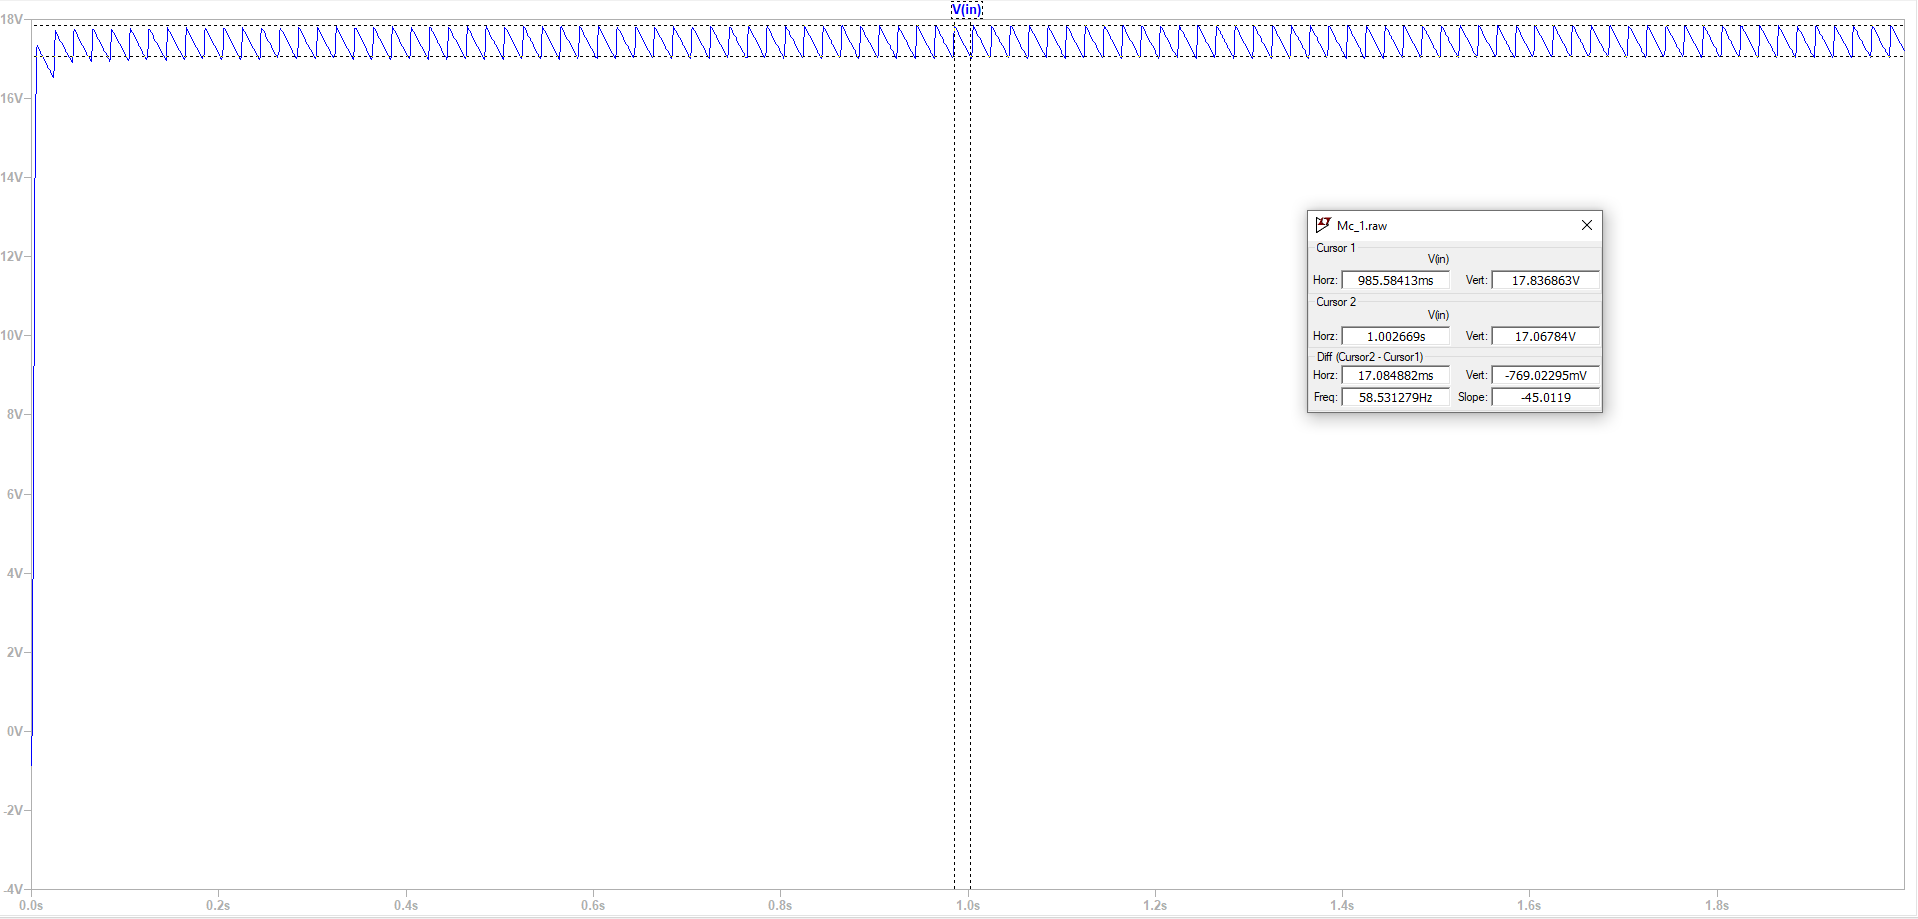
\includegraphics[scale=.4]{Images/3.PNG}}
\caption{V(Out) settling times}
\label{figb}
\end{figure}

A ripple of 769mV around the DC value of 17.44V, i.e., 4.4\%\ , was observed.


\subsection{Sensitivity to input mains variation}

The input voltage of LM7805 (output of rectifier) was plotted for different input voltages.

\begin{figure}[h!]
\centerline{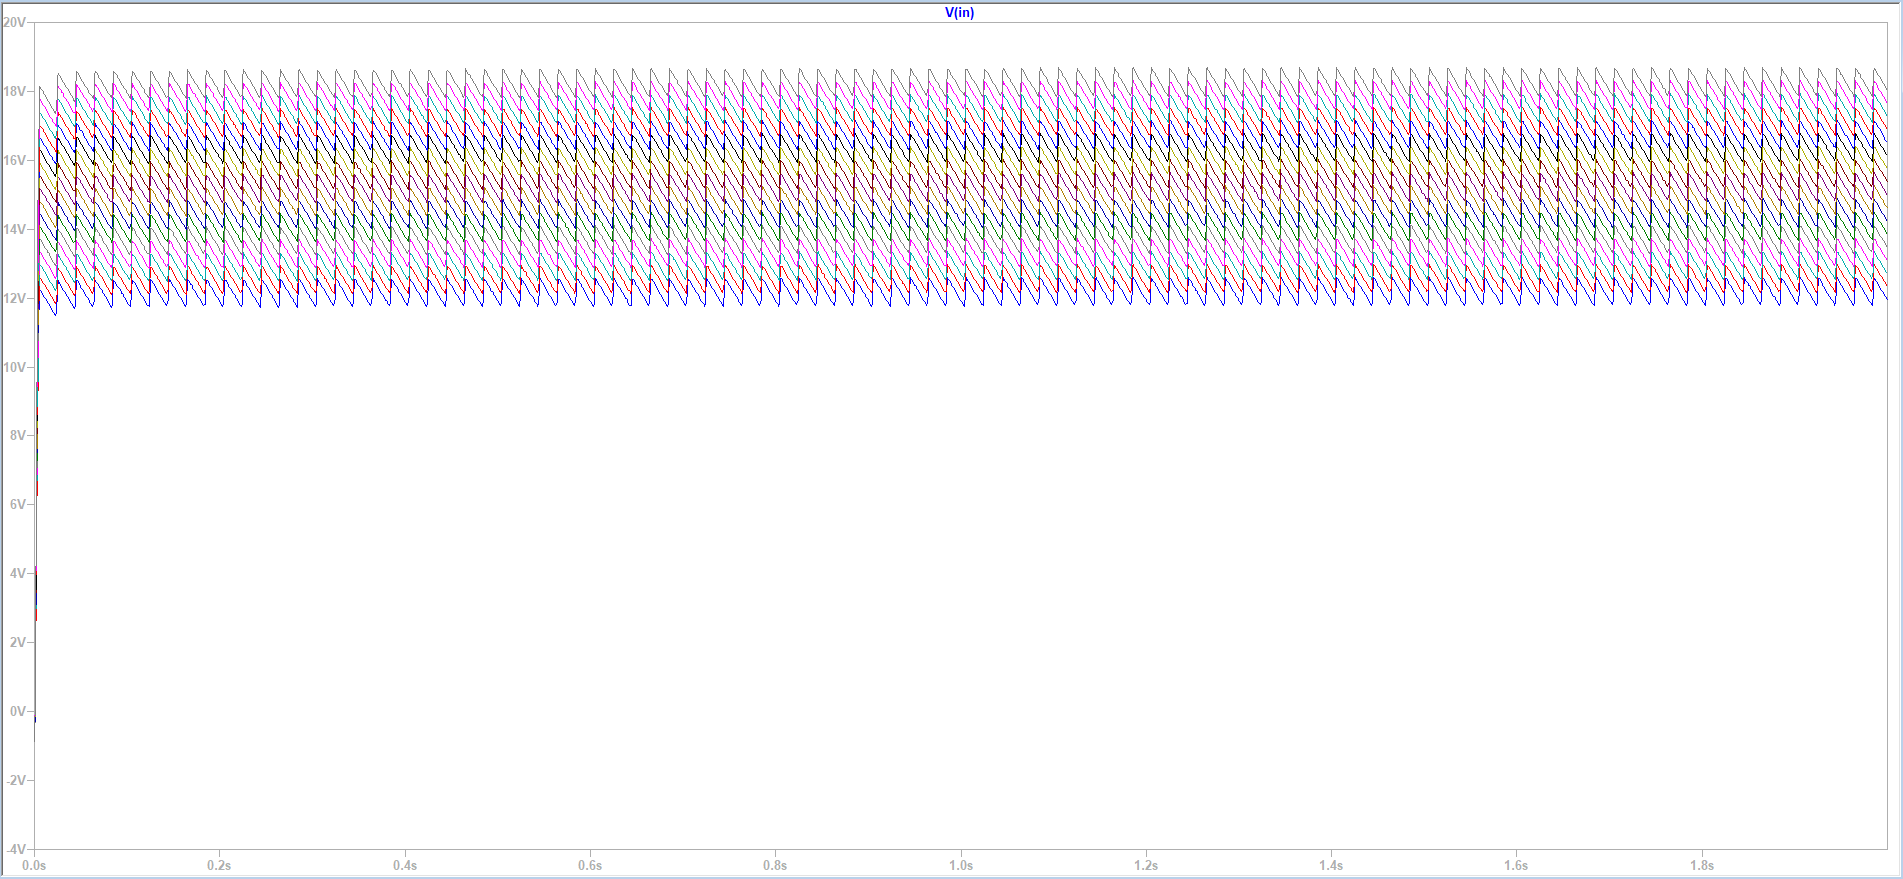
\includegraphics[scale=.4]{Images/4.PNG}}
\caption{V(Out) settling times}
\label{figb}
\end{figure}

The input of the LM7805 has ripples of 5.34\%\ (at 180V (RMS)) or lower. 
\newpage
The output voltage was plotted for the range of input voltages.

\begin{figure}[h!]
\centerline{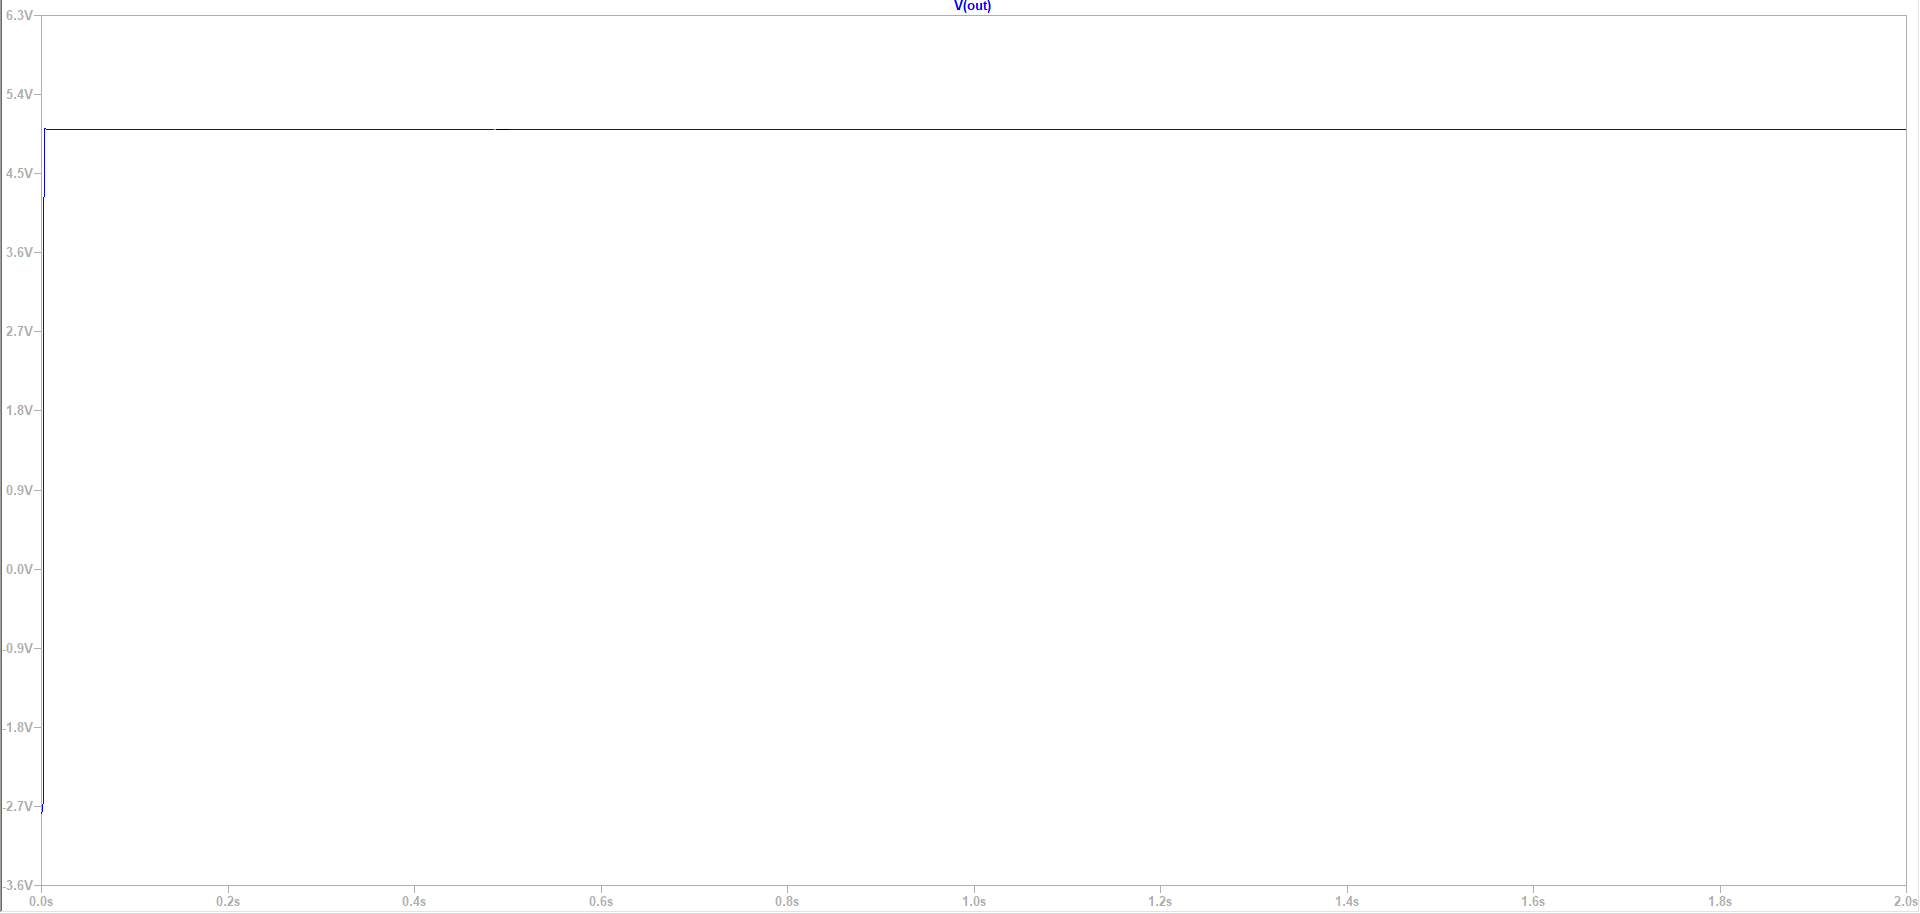
\includegraphics[scale=.4]{Images/5.PNG}}
\caption{V(Out) settling times}
\label{figb}
\end{figure}

 The output voltage, however, settles at a constant 5V DC.

\subsection{Settling time}

The simulation was run for 2.29ms with 230V AC supply voltage. 

\begin{figure}[h!]
\centerline{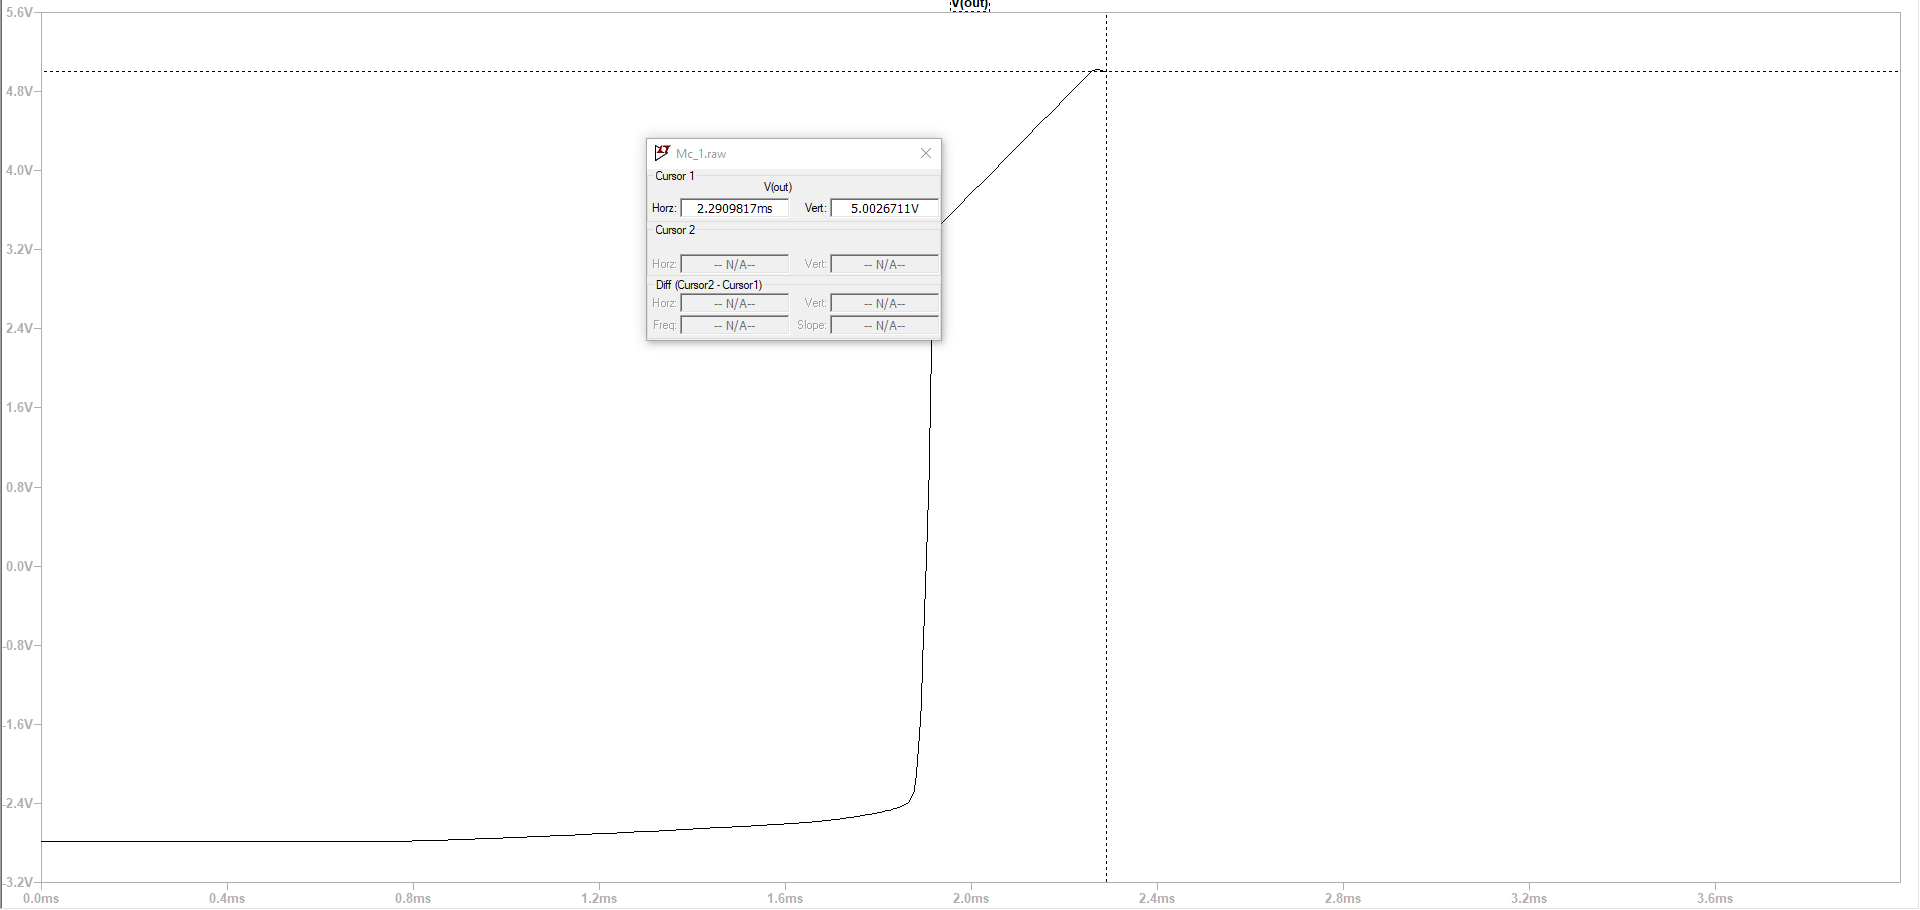
\includegraphics[scale=.4]{Images/6.PNG}}
\caption{V(Out) settling times}
\label{figb}
\end{figure}
The settling time for input voltage of 230V (RMS) AC was found to be around 2.29ms. All of them settle to the same output voltage of 5 V DC.

\newpage
The input voltage (RMS) was sweeped from 180 V to 260 V. The corresponding set of curves of output voltage was plotted across time.

\begin{figure}[h!]
\centerline{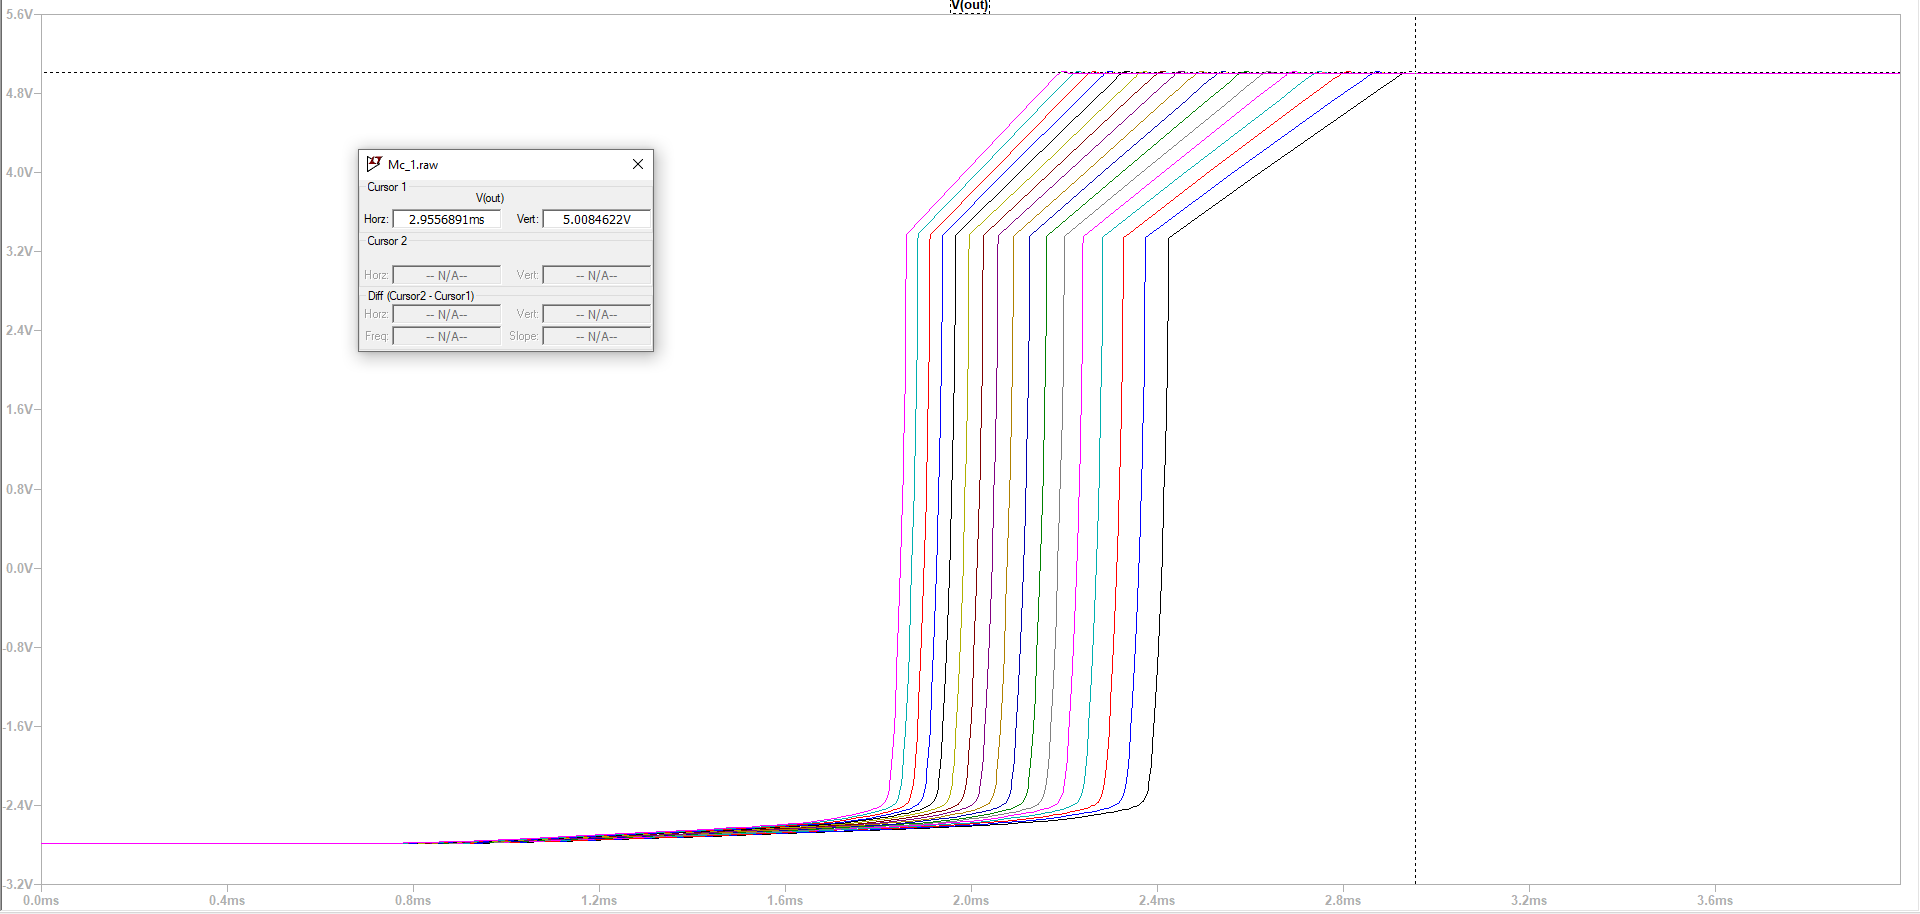
\includegraphics[scale=.4]{Images/7.PNG}}
\caption{V(Out) settling times at different Voltages}
\label{figb}
\end{figure}

The settling time varied from 2.2ms to 3ms.

\section{PCB Design}
% 

\subsection{Layered View Of PCB Layers}
Following are the views of various layers of PCB design. The screw size used is a standard 3.2 mm diameter.

\begin{figure}[h!]
\centerline{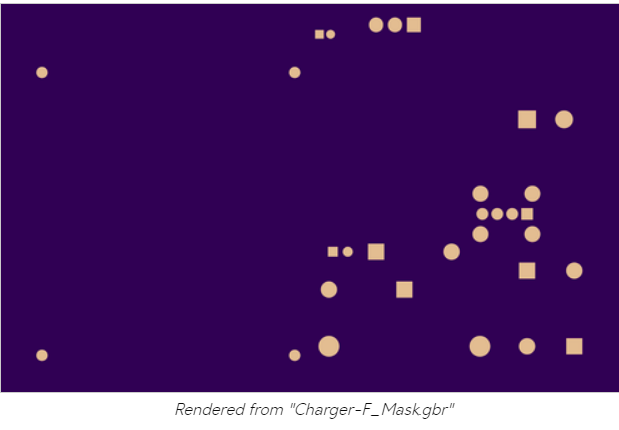
\includegraphics[scale=.8]{Images/u1.png}}
\caption{Top Solder Mask View}
\label{figb}
\end{figure}


\begin{figure}[h!]
\centerline{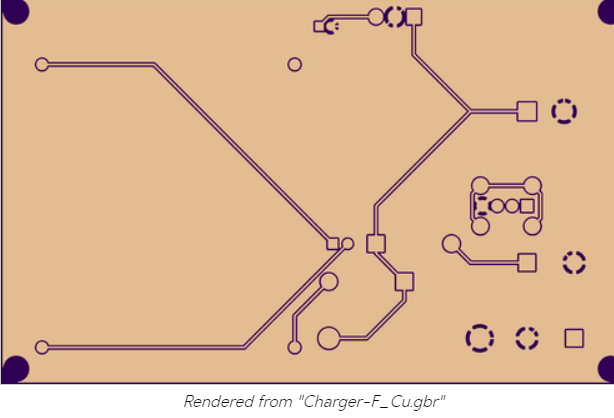
\includegraphics[scale=.6]{Images/u2.png}}
\caption{Top Layer View}
\label{figb}
\end{figure}

\begin{figure}[h!]
\centerline{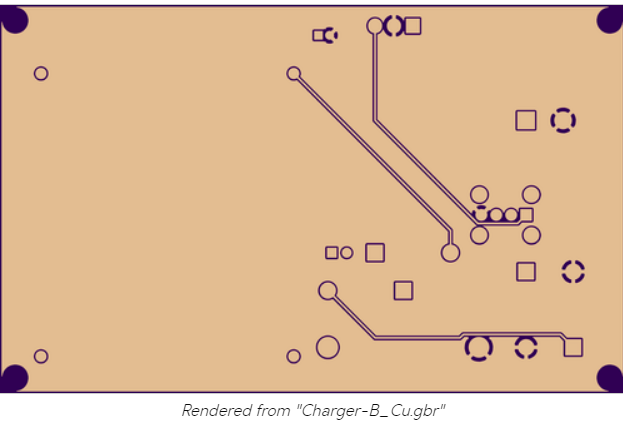
\includegraphics[scale=.6]{Images/u3.png}}
\caption{Bottom Layer View}
\label{figb}
\end{figure}

\begin{figure}[h!]
\centerline{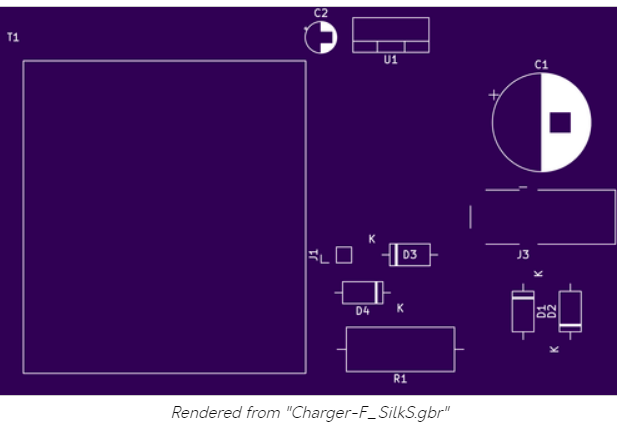
\includegraphics[scale=.6]{Images/u6.png}}
\caption{Top Silk Screen View}
\label{figb}
\end{figure}

\begin{figure}[h!]
\centerline{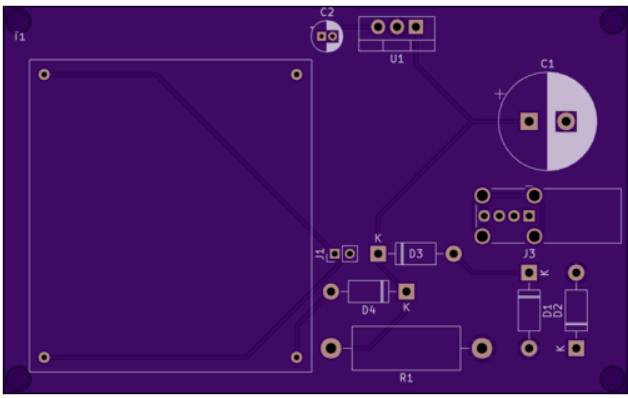
\includegraphics[scale=.6]{Images/u10.png}}
\caption{Board Top}
\label{figb}
\end{figure}

\begin{table}
    \centering
    \begin{tabular}{|l|l|l|}
    \hline
    \multicolumn{3}{|c|}{\textbf{\textit{PCB Footprints}}} \\
    \hline
    \hline
        S.no. & Device Name & Footprint \\ \hline
        1 & C1 & Capacitor\_THT:CP\_Radial\_D13.0mm\_P5.00mm \\ \hline
        2 & C2 & Capacitor\_THT:CP\_Radial\_D4.0mm\_P1.50mm \\ \hline
        3 & D1 & Diode\_THT:DO-41\_SOD81\_P10.16mm\_Horizontal \\ \hline
        4 & D2 & Diode\_THT:DO-41\_SOD81\_P10.16mm\_Horizontal \\ \hline
        5 & D3 & Diode\_THT:DO-41\_SOD81\_P10.16mm\_Horizontal \\ \hline
        6 & D4 & Diode\_THT:DO-41\_SOD81\_P10.16mm\_Horizontal \\ \hline
        7 & J1 & Connector\_PinHeader\_2.00mm:PinHeader\_1$\times$02\_P2.00mm\_Vertical \\ \hline
        8 & J3 & Connector\_USB:USB\_A\_Wuerth\_614004134726\_Horizontal \\ \hline
        9 & R1 & Resistor\_THT:R\_Axial\_DIN0614\_L14.3mm\_D5.7mm\_P20.32mm\_Horizontal\\ \hline
        10 & T1 & Transformer\_:Rectangle\_board\_size38$\times$42mm\_4\_holes\_each\_2mm\_away\_from\_corner \\ \hline
        11 & U1 & Package\_TO\_SOT\_THT:TO-220-3\_Vertical \\ \hline
        
    \end{tabular}
\end{table}
\pagebreak
\newpage

\subsection{3-D View Of PCB}

\begin{figure}[h!]
\centerline{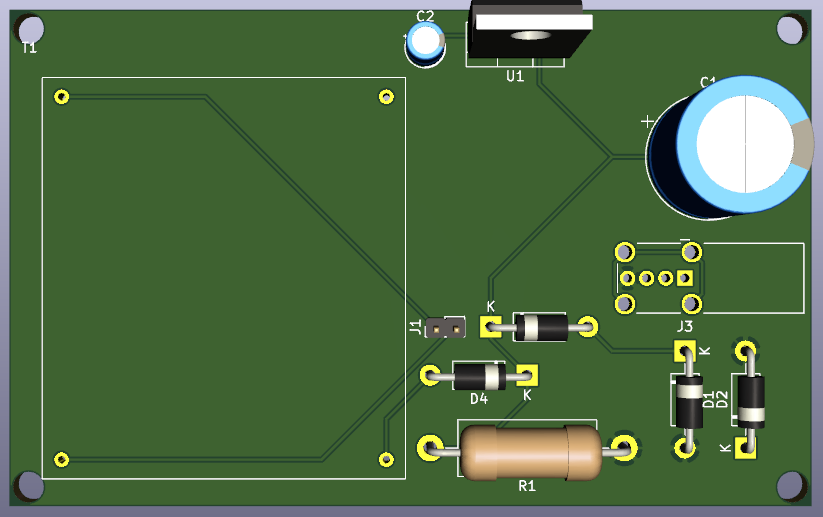
\includegraphics[scale=.6]{Images/a.png}}
\caption{Top 3-D View}
\label{figb}
\end{figure}
\begin{figure}[h!]
\centerline{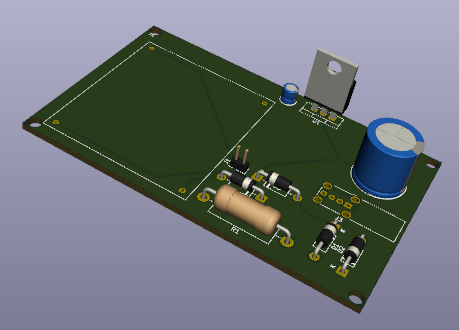
\includegraphics[scale=.8]{Images/final3d.png}}
\caption{Final 3-D View}
\label{figb}
\end{figure}

\begin{figure}[h!]
\centerline{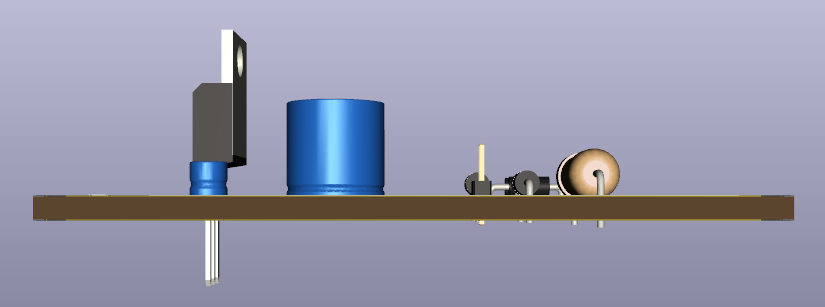
\includegraphics[scale=.6]{Images/c.png}}
\caption{Side 3-D View}
\label{figb}
\end{figure}

\begin{figure}[h!]
\centerline{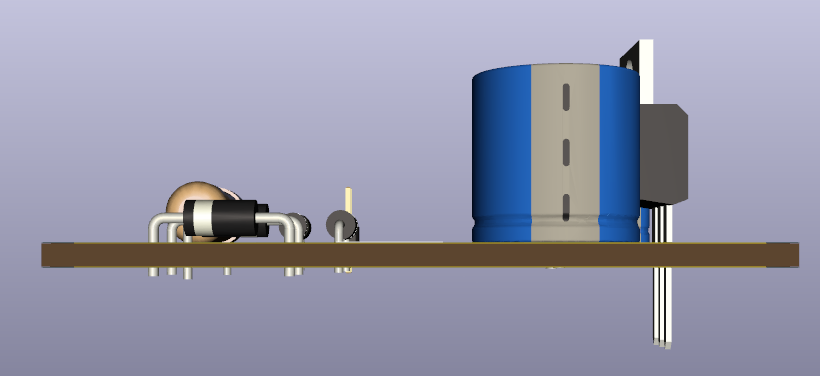
\includegraphics[scale=.6]{Images/d.png}}
\caption{Side 3-D View}
\label{figb}
\end{figure}


\section{Bill of Materials - PCB Cost}

The estimated cost of the proposed PCB is around 200 Rupees. The breakup of cost by parts is done as

\begin{table}
    \centering
    \begin{tabular}{|l|l|l|}
    \hline
    \multicolumn{3}{|c|}{\textbf{\textit{PCB Footprints}}} \\
    \hline
    \hline
        Device & Link to buying Site & Price wrt Quantity \\ \hline
        PCB                 & \cite{noauthor_1_cost_nodate} & 15.5 (Rs. 100/ sq. inch) \\
        1u                  & \cite{noauthor_2_cost_nodate} & 10.53 (per 5 cap)        \\
        22m                 & \cite{noauthor_3_cost_nodate} & 14                       \\
        1N4007              & \cite{noauthor_4_cost_nodate} & 40 (per 50 pcs)          \\
        Conn\_01x02\_Male   & \cite{noauthor_5_cost_nodate} & 9 per 40 pins            \\
        USB\_A female       & \cite{noauthor_6_cost_nodate} & 15                       \\
        20Meg               & \cite{noauthor_7_cost_nodate} & 0.7                      \\
        Transformer\_1P\_1S & \cite{noauthor_8_cost_nodate} & 99                       \\
        LM7805\_TO220       & \cite{noauthor_9_cost_nodate} & 9 \\
        \hline
        
    \end{tabular}
\end{table}

Taking into account a bit more expenses for soldering and fabrication etc, the total cost comes around \textbf{200 Rupees}, which is an upper limit. The most expensive component is the Transformer.

\newpage

\section{Heating Problem - A Heat Sink}
The PCB has been made keeping in mind that the LM7805 Element can get heated up to high temperatures. To counteract that, we use the following heat dissipating heat sink

\begin{figure}[h!]
\centerline{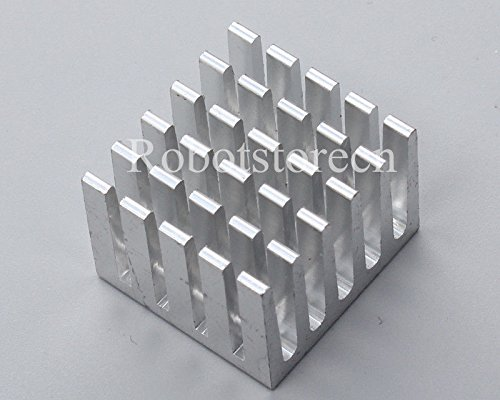
\includegraphics[scale=.3]{Images/51y0tmVtm2L.jpg}}
\caption{The Proposed Heat Sink}
\label{figb}
\end{figure}

The dimension of this heat sink is 20x20x15 mm\cite{noauthor_heat_nodate}, which is an exact fit for our circuit. Another option will be to use a smaller heat sink

\begin{figure}[h!]
\centerline{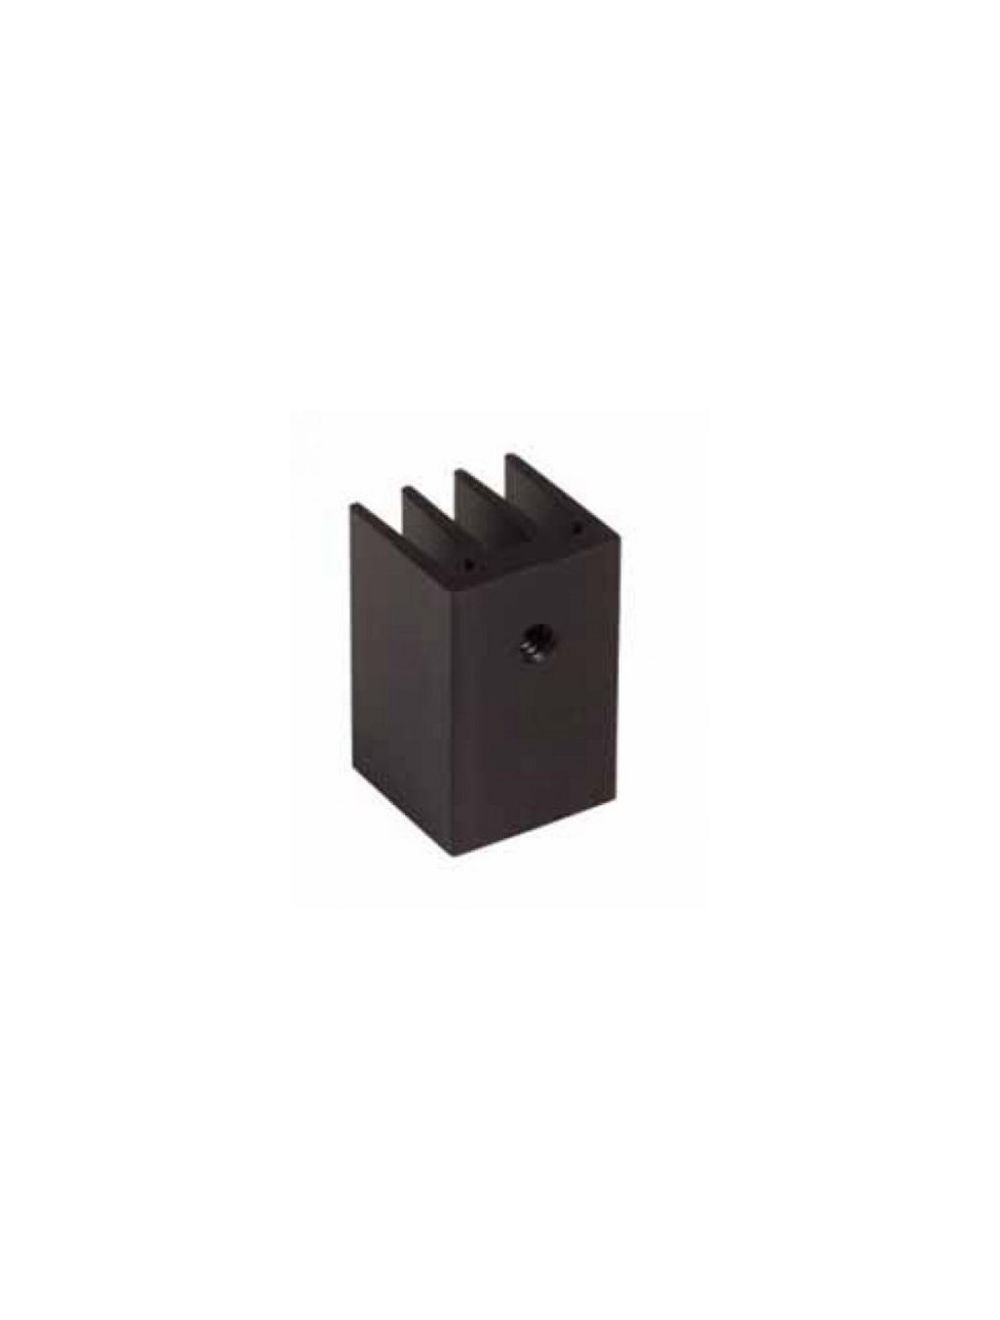
\includegraphics[scale=.25]{Images/heat-sink-pi49-500x500.jpg}}
\caption{Another Heat Sink}
\label{figb}
\end{figure}

This is a smaller, but less effective heat sink\cite{noauthor_heat_nodate}

\newpage
\section{Conclusions}

A mobile charger delivering 1A current at constant 5V DC was designed and simulated on LTSpice using relatively cheap and commercially available circuit elements and it's model was implemented on PCB using KiCad . The specifications have been met as far as possible.



\printbibliography

\end{document}
